The parameters of the orbits analysed in the simulator are presented in \autoref{tab:orbits}.

\begin{table}[ht]
	\centering
	\begin{tabular}{ccc}
	\toprule
	& Tundra & Molniya\\
	\midrule
	Orbital Period (s)     & 86400   & 43200\\
	Eccentricity        & 0.25   & 0.71\\
	Semi-major axis (km) & 42164 & 26556\\
	Inclination (deg)      & 63.4 & 63.4\\
	Initial RAAN (deg)	& 120	& 25\\
	\bottomrule
	\end{tabular}
	\caption{Parameters of the considered orbits}
	\label{tab:orbits}
\end{table}

In the simulation, two equally spaced satellites were used: when the first one is in the apogee, the other one is in the perigee and moreover the \gls{raan}'s offset between satellites is $90^\circ$ for Molniya and $180^\circ$ for Tundra.
As it is shown in \autoref{fig:molniya} and \autoref{fig:tundra}, each satellite has its own orbital plane, but the resulting ground track for the different satellites is the same.

Since Molniya's period is half of the revolution period of the Earth, we simulated two revolutions of the satellites around the Earth so to make it easier to understand the figures.
For Tundra, on the other hand, one revolution around the Earth is enough since this orbit is Geosynchronous.

\begin{figure}[!htbp]
	\begin{subfigure}{.5\textwidth}
	\centering
	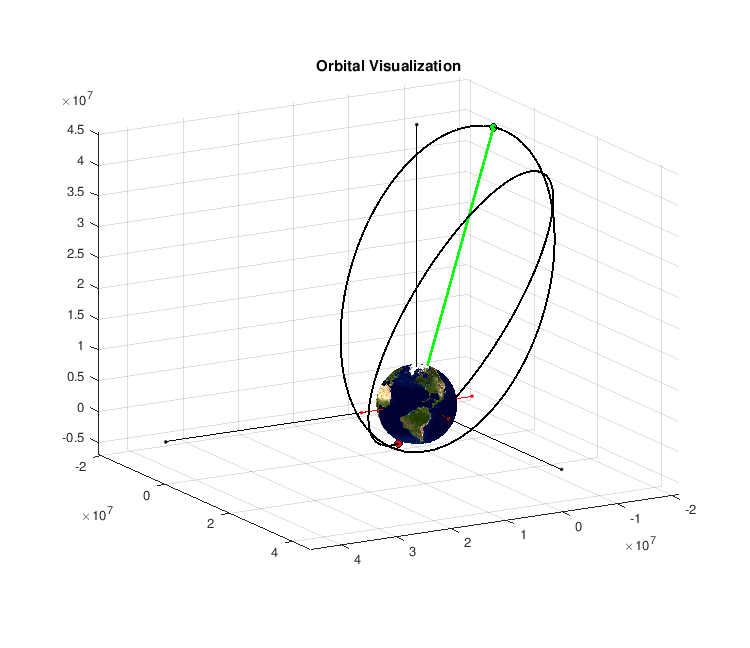
\includegraphics[width = \textwidth]{3D_molniya.png}
	\caption{3D Visualization}
	\label{fig:3D_molniya}
	\end{subfigure}
	\begin{subfigure}{.5\textwidth}
	\centering
	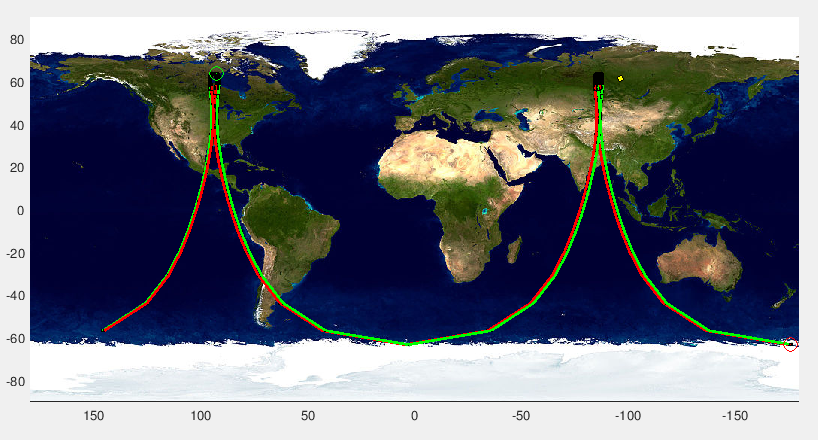
\includegraphics[width = \textwidth]{GT_molniya.png}
	\caption{Ground Track}
	\label{fig:GT_molniya}
	\end{subfigure}
	\caption{Graphical visualization of Molniya orbit}
	\label{fig:molniya}
\end{figure}

\begin{figure}[!htbp]
	\begin{subfigure}{.5\textwidth}
	\centering
	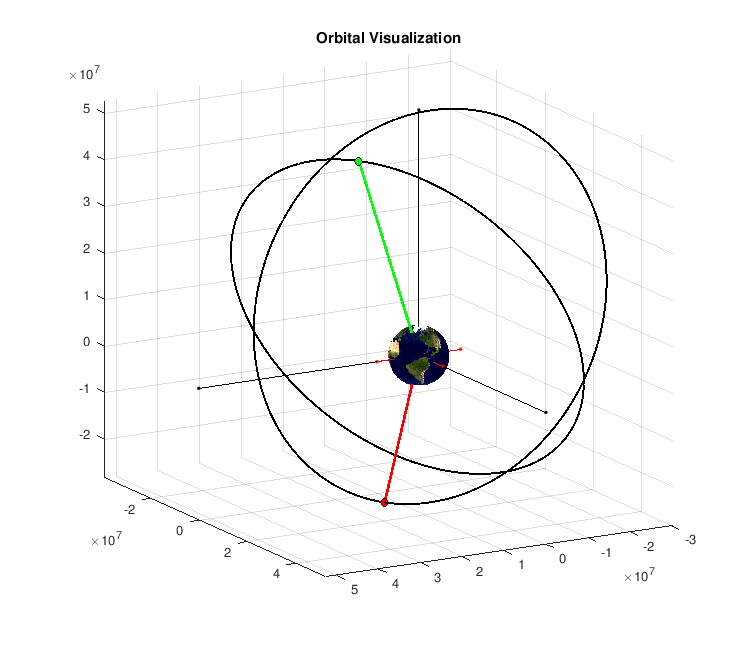
\includegraphics[width = \textwidth]{3D_tundra.png}
	\caption{3D Visualization}
	\label{fig:3D_tundra}
	\end{subfigure}
	\begin{subfigure}{.5\textwidth}
	\centering
	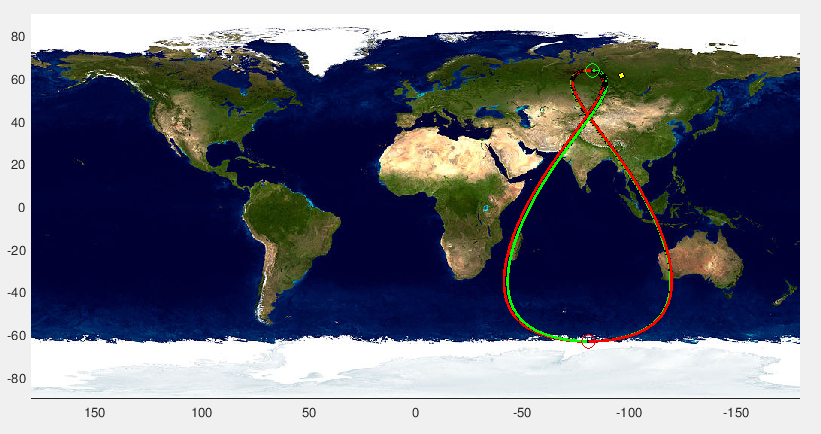
\includegraphics[width = \textwidth]{GT_tundra.png}
	\caption{Ground Track}
	\label{fig:GT_tundra}
	\end{subfigure}
	\caption{Graphical visualization of Tundra orbit}
	\label{fig:tundra}
\end{figure}

Plotting the azimuth and the elevation for different positions in the service area (\autoref{fig:elevation_multi}), the result is that the elevation with a Molniya Orbit is higher, on average. In some cases, the advantage of Molniya is not so visible from the elevation plots, but in the end the Link Budget gives higher values for Molniya than for Tundra.

For all these reasons, we chose to adopt a Molniya orbit with the parameters set as in \autoref{tab:orbits} for our system.

\begin{figure}[!htbp]
	\begin{subfigure}{.5\textwidth}
	\centering
	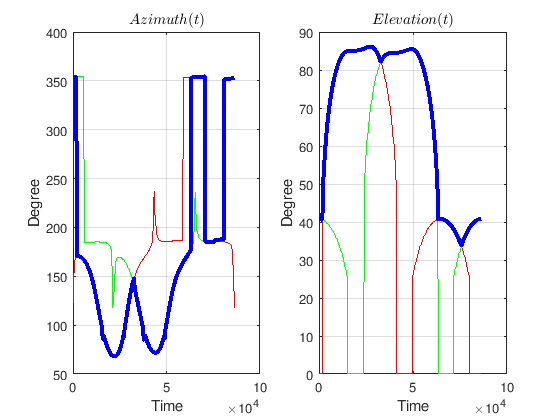
\includegraphics[width = \textwidth]{AZEL_molniya_lat61_long-75.png}
	\caption{Molniya, $Lat = 61^\circ ~ Long = -75^\circ$}
	\end{subfigure}
	\begin{subfigure}{.5\textwidth}
	\centering
	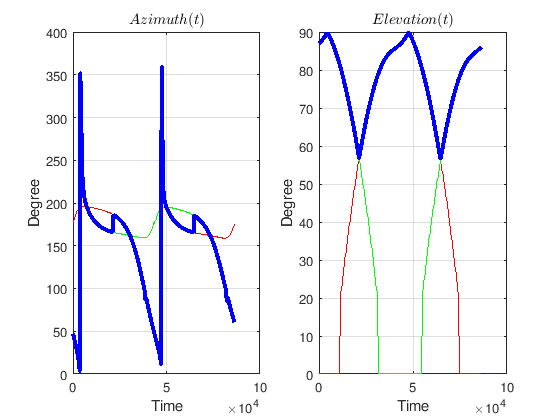
\includegraphics[width = \textwidth]{AZEL_tundra_lat61_long-75.png}
	\caption{Tundra, $Lat = 61^\circ ~ Long = -75^\circ$}
	\end{subfigure}
	\vspace{0.5cm}
	\begin{subfigure}{.5\textwidth}
	\centering
	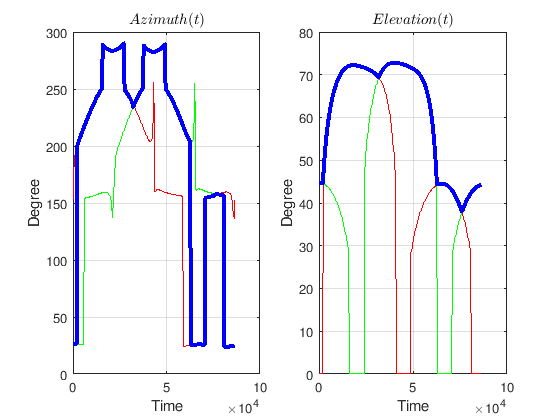
\includegraphics[width = \textwidth]{AZEL_molniya_lat61_long-130.png}
	\caption{Molniya, $Lat = 61^\circ ~ Long = -130^\circ$}
	\end{subfigure}
	\begin{subfigure}{.5\textwidth}
	\centering
	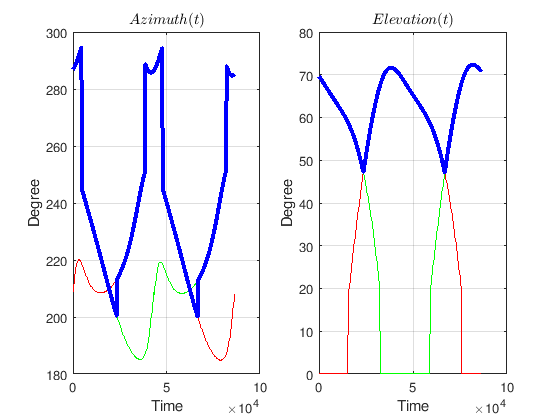
\includegraphics[width = \textwidth]{AZEL_tundra_lat61_long-130.png}
	\caption{Tundra, $Lat = 61^\circ ~ Long = -130^\circ$}
	\end{subfigure}
	\end{figure}
	\begin{figure}[!htbp]\ContinuedFloat
	\begin{subfigure}{.5\textwidth}
	\centering
	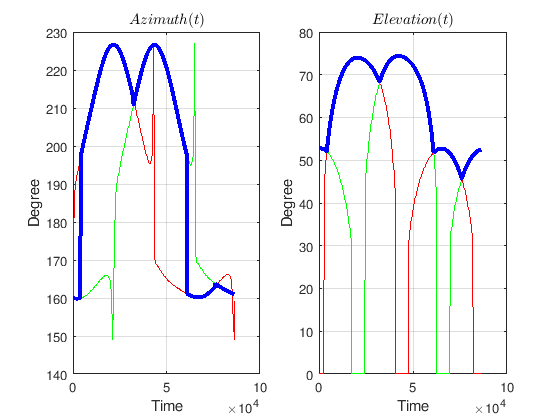
\includegraphics[width = \textwidth]{AZEL_molniya_lat71_long-130.png}
	\caption{Molniya, $Lat = 71^\circ ~ Long = -130^\circ$}
	\end{subfigure}
	\begin{subfigure}{.5\textwidth}
	\centering
	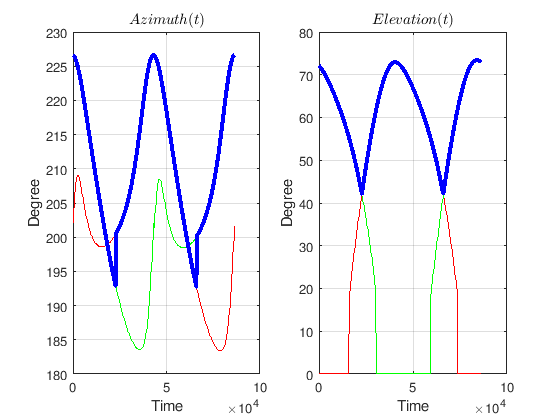
\includegraphics[width = \textwidth]{AZEL_tundra_lat71_long-130.png}
	\caption{Tundra, $Lat = 71^\circ ~ Long = -130^\circ$}
	\end{subfigure}
	\vspace{0.5cm}
	\begin{subfigure}{.5\textwidth}
	\centering
	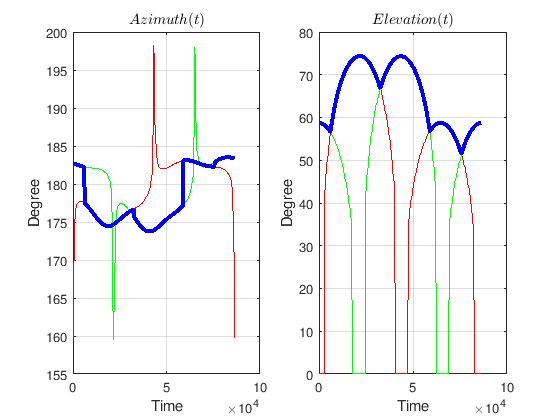
\includegraphics[width = \textwidth]{AZEL_molniya_lat81_long-75.png}
	\caption{Molniya, $Lat = 81^\circ ~ Long = -75^\circ$}
	\end{subfigure}
	\begin{subfigure}{.5\textwidth}
	\centering
	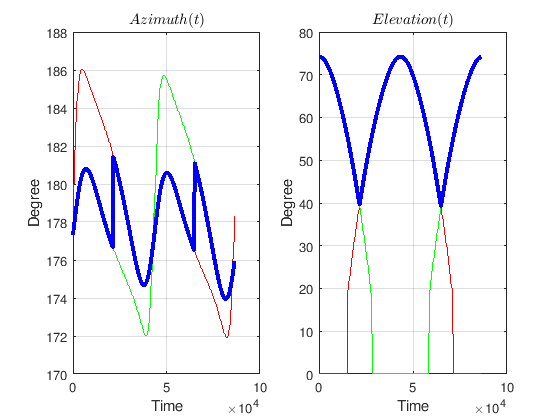
\includegraphics[width = \textwidth]{AZEL_tundra_lat81_long-75.png}
	\caption{Tundra, $Lat = 81^\circ ~ Long = -75^\circ$}
	\end{subfigure}
	\vspace{0.5cm}
	\begin{subfigure}{.5\textwidth}
	\centering
	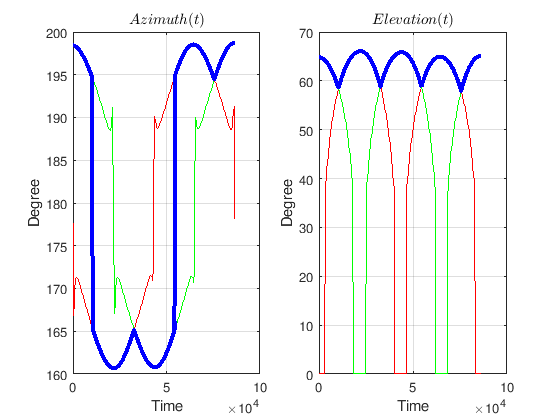
\includegraphics[width = \textwidth]{AZEL_molniya_lat81_long0.png}
	\caption{Molniya, $Lat = 81^\circ ~ Long = 0^\circ$}
	\end{subfigure}
	\begin{subfigure}{.5\textwidth}
	\centering
	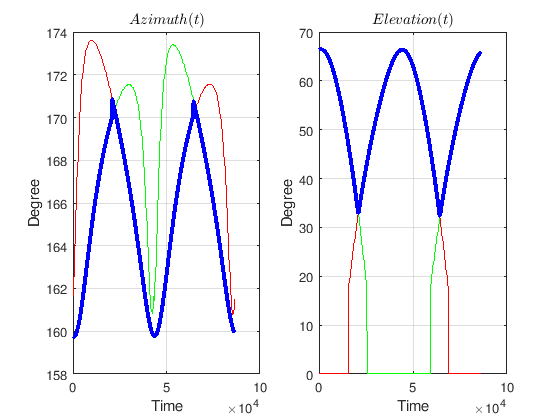
\includegraphics[width = \textwidth]{AZEL_tundra_lat81_long0.png}
	\caption{Tundra, $Lat = 81^\circ ~ Long = 0^\circ$}
	\end{subfigure}
	\caption{Elevation and Azimuth for different position in the service area of Molniya and Tundra orbits}
	\label{fig:elevation_multi}
\end{figure}

\newpage
